\documentclass[
    a4paper,
    man,
    floatsintext
]{style}
\usepackage[T1]{fontenc}
\usepackage[american]{babel}
\usepackage[style=apa,backend=biber,sorting=nyt]{biblatex}
\NewBibliographyString{unpublished}
\DefineBibliographyStrings{english}{
  unpublished = {Unpublished},
}
\DefineBibliographyStrings{american}{
  unpublished = {Unpublished},
}
\usepackage[font={footnotesize,it}]{caption}
\usepackage{csquotes}
\usepackage{booktabs} 
\usepackage{tabularx}
\usepackage{linguex} 
\usepackage{filestyle}
\usepackage{amsmath}
\usepackage{graphicx}
\graphicspath{ {./graphics/} }
%\usepackage{times}
\usepackage{ragged2e}
\usepackage{hyperref}
\usepackage{enumitem}
\newcommand{\quotes}[1]{``#1''}
\usepackage[title]{appendix}
\usepackage{booktabs}
\providecommand{\firstrefdash}{} %removes dash in references to examples, i.e. (1a) instead of (1-a)
\addbibresource{sample.bib}
\addbibresource{references.bib}
%%%%%%%%%%%%%%%%%%%%%%%%%%%%%%%%%%%%%%%%%%%%%%%%%%%
\title[Title]{Title}
\author[Author1, Author2] % LEAVE ANONYMOUS
{\spauthor{Luca Luigi Alberici\\
  \institute{Bayes Business School}
  \small{luca-luigi.alberici@bayes.city.ac.uk}
  }
  \AND
\spauthor{Nawfal Khodabacchas\\
  \institute{Coverys Limited}\\
  \small{nawfal.khodabacchas@coverys.co.uk}
  }
\AND
\spauthor{Lina Palacios\\
  \institute{LeWagon GmbH}\\
  \small{linam.palacios@gmail.com}
  }
\AND
\spauthor{Sarah MacDonnell\\
  \institute{LCP}\\
  \small{sarah.macdonnell@lcp.com}
  }
}

\begin{document}
\maketitle

\begin{abstract}
The abstract text goes here.
\end{abstract}

\begin{keywords}
  keyword 1; keyword 2; keyword 3; keyword 4
\end{keywords}

\section{Introduction}
\label{intro}

Loss reserving is, at its core, an exercise in managing heterogeneity. Claims differ in size, in the delay before they are reported, in the time they take to settle, and in the pattern of payments and case-estimate revisions they generate. Traditional methods deal with this by aggregating claims into run-off triangles, segmented in advance by line of business, type of cover or accident period, and by assuming that development is homogeneous within each segment \parencite{taylor2000loss,england2002stochastic}. The segments are chosen by judgement, and the plausibility of the homogeneity assumption depends on how well that judgement was made.

Recent research has turned to individual-claim data and machine-learning methods \parencite{wuthrich2018machine}, supported by simulators that generate claim histories whose properties are fully known \parencite{avanzi2021synthetic,avanzi2023splice}. Within this landscape, unsupervised clustering is an appealing tool. Rather than imposing segments, it lets the data suggest groups of claims, or of portfolio cohorts, with similar development characteristics. Such groups could support segmentation \emph{before} reserving, or help to interpret the results of a reserving analysis. This is the question we investigate: can clustering claims by their development characteristics yield segments that are useful to a reserving actuary?

Clustering is, however, unforgiving in a specific way. It has no target variable, so there is no held-out error to tell us whether the result is right. K-means, hierarchical and model-based algorithms will return a partition of any data set, and that partition depends on decisions taken before the algorithm is run: what counts as an object (a claim or an occurrence period), which variables describe it, on what scale, under which distance and into how many groups \parencite{jain2010data,hastie2009elements}. Each of those decisions can be defended only with knowledge of the data. An analyst who skips the data-understanding stage does not avoid making them; the analyst makes them implicitly, and without evidence.

This paper therefore treats understanding the data as the first stage of the clustering study, not as a preliminary to it. Using the SPLICE Complexity~5 portfolio \parencite{avanzi2023splice}, we validate the structure of the data, examine the distribution of the candidate features and the dependence between them, and choose the unit of analysis. Our aim is twofold: to report the features of the data that matter for reserving, and to show that each of them translates into a concrete modelling decision, from the transformation of variables to the choice of algorithm. Section~\ref{theory} sets out the theoretical background, Section~\ref{data} presents the data and the exploratory analysis, and Section~\ref{methodology} describes the clustering methodology that builds on them.

\section{Theoretical Background}
\label{theory}
\section{Data and Exploratory Analysis}
\label{data}

Before any clustering algorithm is run, the analyst must decide what is being clustered, on what scale and with which variables. This section documents those decisions for the SPLICE Complexity~5 portfolio (original analysis: \texttt{notebooks/01\_data\_exploration.ipynb}; figures and supplementary checks: \texttt{article/make\_figures.py}).

\subsection{Why understanding the data comes first}
\label{sec:why}

Clustering is often described as letting the data speak. In practice the data speak only through the analyst's preparation of them, and four considerations explain why that preparation has to be informed.

First, clustering algorithms always return an answer. K-means, hierarchical and model-based methods will partition any data set into the requested number of groups, whether or not it contains natural groups, and without a target variable there is no held-out error to say whether the result is meaningful \parencite{jain2010data}. Second, distance-based methods are sensitive to the scale, skewness and redundancy of their inputs. A variable spanning six orders of magnitude swamps one that counts payments, a few extreme observations can pull centroids towards them, and several variables that measure the same phenomenon give it several votes; even the choice of standardisation can materially change how well structure is recovered \parencite{milligan1988study,hastie2009elements}. Third, the unit of analysis and the timing of information determine what a cluster \emph{means}. A cluster of completed claims describes history, whereas a cluster of open claims at a valuation date can support prediction, and mixing the two is a form of information leakage \parencite{kaufman2012leakage}. Fourth, data errors do not stay local: a broken link between tables or a misread missing value is absorbed silently into the features, so the clusters reflect the plumbing of the data rather than the behaviour of claims.

\emph{Practical implication.} Reserving practice already rests on reconciliation and on knowing what is available at the valuation date; what changes is that, with nothing to fit, no residual warns us that a preparation choice was wrong. Exploratory work is therefore part of the model \parencite{tukey1977exploratory}, since summary statistics alone can conceal the structure that matters \parencite{anscombe1973graphs}.

\subsection{The SPLICE Complexity 5 portfolio}
\label{sec:splice}

We use SPLICE, a simulator of individual claim histories that models payments and the evolution of case estimates \parencite{avanzi2023splice}, built on the SynthETIC claim simulator \parencite{avanzi2021synthetic}. Simulated data suit a first study because they are complete and because the mechanisms that generate heterogeneity are known, which will later let us check whether clusters recover something real. The price is realism: conclusions will need confirming on real data.

We take the Complexity~5 scenario (random seed 42) from the example data distributed with SPLICE.\footnote{\url{https://github.com/agi-lab/SPLICE}, folder \texttt{datasets/complexity\_5}.} It is the most complex of the five published scenarios, with dependence between claim size and both delays, and between settlement delay and occurrence period. The portfolio has 3,663 claims from 40 quarterly occurrence periods, held in three tables linked by the claim identifier: claims (one row per claim), payments (19,322 rows) and incurred transactions (31,554 rows, recording case-estimate revisions and cumulative payments). Times are in quarters; amounts are in unspecified currency units.

\subsection{Structural validation}
\label{sec:validation}

We validated the tables before examining any distribution, leaving the raw values unmodified. The claim identifier is unique, all 3,663 claims appear in both transaction tables, no transaction refers to an unknown claim, and the number of payment records per claim agrees with the recorded number of payments in every case. The only missing entries are 9,593 revision multipliers in the incurred table, which are structural rather than defects: they coincide exactly with the payment-only transactions, in which no case-estimate revision occurs. The nominal payments of each claim also sum to its recorded claim size to numerical precision. The tables therefore form a coherent relational data set, and no imputation or repair is needed.

\subsection{Marginal distributions}
\label{sec:marginals}

Our baseline description of a claim uses four variables from the claims table: claim size (ultimate severity), notification delay, settlement delay and the number of payments, which capture how large a claim is, how quickly it is reported, how long it takes to settle and how many payments it involves (Table~\ref{tab:desc}, Figure~\ref{fig:dist}).

\begin{table}[!htbp]
\centering
\small
\caption{Descriptive statistics of the candidate clustering variables ($n = 3{,}663$), with skewness on the raw scale and after a $\log(1+x)$ transformation.}
\label{tab:desc}
\begin{tabular}{@{}lrrrrrr@{}}
\toprule
 & & & & & \multicolumn{2}{c}{Skewness} \\
\cmidrule(l){6-7}
Variable & Mean & Median & 95th pct. & Maximum & Raw & Log \\
\midrule
Claim size & 166,924 & 77,185 & 618,724 & 3,130,790 & 3.69 & $-1.01$ \\
Notification delay & 2.14 & 1.74 & 5.37 & 12.13 & 1.36 & 0.17 \\
Settlement delay & 9.80 & 7.55 & 27.23 & 56.29 & 1.37 & $-0.31$ \\
Number of payments & 5.27 & 4 & 11 & 30 & 2.13 & $-0.03$ \\
\bottomrule
\end{tabular}
\end{table}

\begin{figure}[!htbp]
\centering
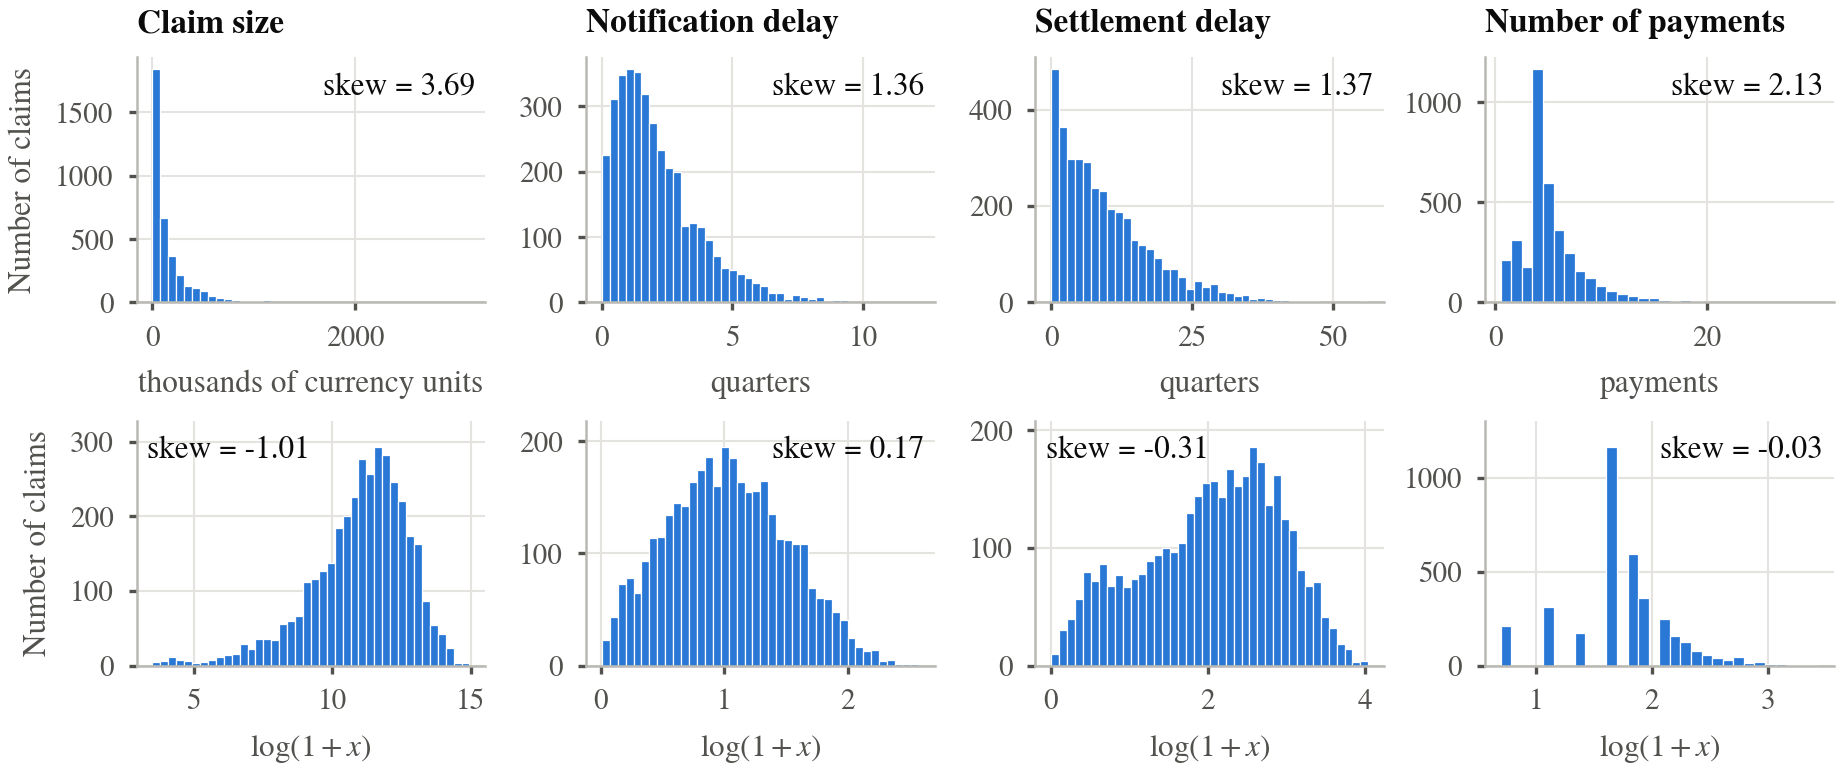
\includegraphics[width=0.95\textwidth]{fig_distributions.png}
\caption{Marginal distributions of the four candidate variables on the raw scale (top) and after a $\log(1+x)$ transformation (bottom), with sample skewness.}
\label{fig:dist}
\end{figure}

All four variables are right-skewed and measured on very different scales. Claim size is the most extreme: its mean is more than twice its median, the largest claim is about 41 times the median claim, and the largest 10\% of claims account for 46\% of total claim cost. Euclidean distance on the raw variables would let claim size decide almost every distance. A $\log(1+x)$ transformation reduces the skewness of every variable to about one or less in absolute value, and standardisation then puts them on a comparable footing.

The logarithm is not a cure-all, however. For claim size it slightly over-corrects, leaving a left tail of very small claims (116 below 1,000, of which 27 below 100). Log settlement delay has a shoulder at short delays, hinting at a group of quickly settled claims (Section~\ref{sec:dependence}). The number of payments is discrete, with a sharp mode at four payments (1,166 claims, about a third), so no transformation makes it look continuous. The extreme claims are valid simulated observations and we retain them: in reserving, large and long-tailed claims are often exactly the segment of interest. \emph{Practical implication:} transform and standardise before computing any distance, but do not delete the tail; assess its influence by sensitivity analysis instead.

\subsection{Dependence between candidate features}
\label{sec:dependence}

Because the variables are skewed and one is discrete, we measure dependence with Spearman rank correlation (Figure~\ref{fig:dep}a). Claim size is strongly associated with both settlement delay ($\rho = 0.68$) and the number of payments ($\rho = 0.68$), and settlement delay with the number of payments ($\rho = 0.54$). Notification delay is weakly and negatively related to the others ($\rho$ between $-0.29$ and $-0.19$). The Pearson correlations for the first three pairs are markedly lower (0.45, 0.39, 0.37), so the relationships are monotone but far from linear: larger claims stay open longer and involve more payments.

\begin{figure}[!htbp]
\centering
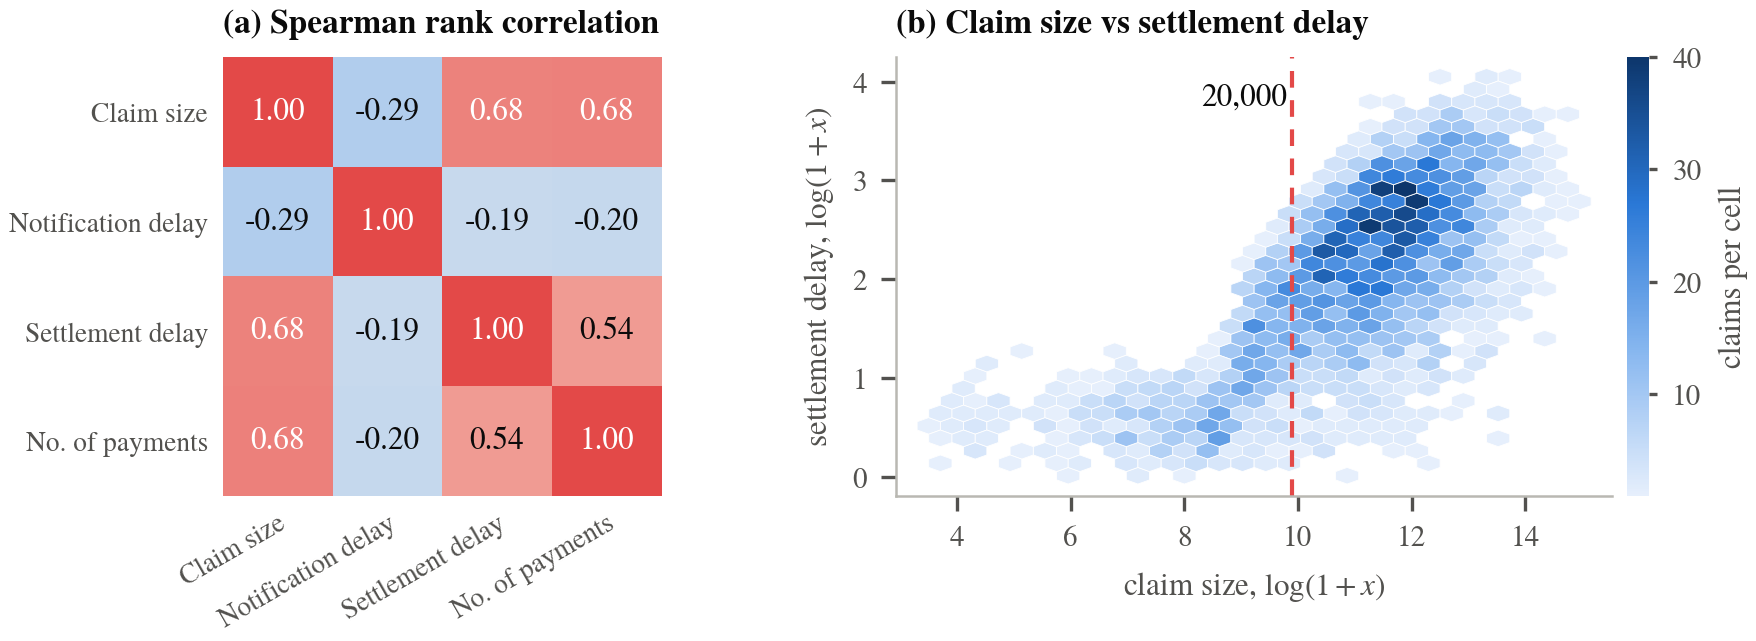
\includegraphics[width=0.95\textwidth]{fig_dependence.png}
\caption{(a)~Spearman rank correlations between the candidate variables. (b)~Claim size against settlement delay on the $\log(1+x)$ scale; the dashed line marks a claim size of 20,000.}
\label{fig:dep}
\end{figure}

Claim size, settlement delay and the number of payments are therefore largely three measurements of one dimension, which one might call claim complexity. Under equal-weight distances that dimension is counted three times, and clusters are likely to be organised around it. We keep the four variables at first but plan a sensitivity analysis over alternative feature subsets.

Figure~\ref{fig:dep}b shows a second feature that the correlation matrix hides: the joint distribution is not a single elliptical cloud. Claims below roughly 20,000 (833 claims, 23\% of the portfolio) settle far more quickly than the rest, with a median settlement delay of 1.4 quarters against 10.2, and form a distinct band of short delays rather than the lower end of the main cloud. This is consistent with the scenario's specification (mean settlement delay grows with the logarithm of claim size) and explains the shoulder in Figure~\ref{fig:dist}. It matters because K-means favours compact, roughly spherical groups \parencite{hastie2009elements}, so shapes like this argue for also using hierarchical and model-based clustering.

\subsection{Choosing the unit of analysis}
\label{sec:unit}

A reserving analyst can cluster individual claims or aggregated portfolio cohorts, and the choice changes the question being asked. The cohort alternative is to summarise each occurrence period by its claim frequency and typical claim characteristics and to look for periods that behave alike. We built this period-level table (40 rows) and examined it for regimes (Figure~\ref{fig:periods}). Claim frequency ranges from 73 to 111 claims per period (mean 91.6), and the median claim size, median settlement delay and mean number of payments fluctuate around stable levels without persistent breaks. The only visible drift is a mild fall in settlement delay across periods (Spearman correlation of $-0.06$ with occurrence period), consistent with the scenario's design. Period-level clustering would also cut the sample from 3,663 observations to 40 and would conceal the claim-level heterogeneity seen above: the share of claims below 20,000 is essentially constant over time (22\% in periods 1--20, 23\% in periods 21--40), so period medians barely register the quick-settling group.

\begin{figure}[!htbp]
\centering
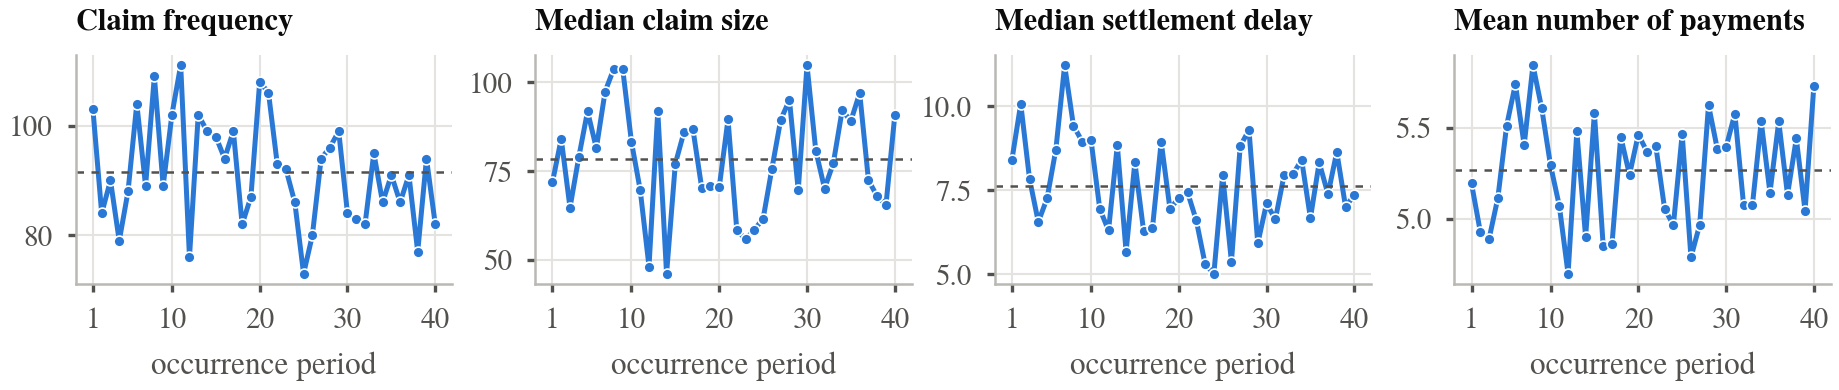
\includegraphics[width=0.9\textwidth]{fig_periods.png}
\caption{Occurrence-period summaries (40 periods); the dashed line is the average over periods. Claim size is in thousands of currency units and settlement delay in quarters.}
\label{fig:periods}
\end{figure}

We therefore take the individual claim as the primary unit of analysis, since it gives enough observations and preserves variation between claims; occurrence-period summaries remain a secondary diagnostic for the resulting clusters.

\subsection{An ex-post baseline}
\label{sec:expost}

The baseline variables include ultimate claim size, final settlement delay and final number of payments, none of which is known until a claim has settled. Our first clustering exercise is consequently an \emph{ex-post segmentation}: it can describe different types of completed claim, but it cannot assign a claim to a cluster at notification or at a valuation date. A reserving application must separate features available at the valuation date from the outcomes the analysis is meant to understand or predict \parencite{kaufman2012leakage}. Aggregating the payment and incurred tables to one row per claim can supply such features, for example time to first payment, proportion paid at given development ages, and the number and size of incurred revisions. The covariate-adjusted portfolio (files with suffix \texttt{\_cov}) is a separate simulation, kept for robustness checks.

\subsection{From findings to design decisions}
\label{sec:decisions}

Table~\ref{tab:decisions} traces each finding to a design decision. None is exotic, but each is invisible to the algorithm and consequential for its output, so documenting them lets the results that follow be interpreted and challenged.

\begin{center}
\footnotesize
\captionof{table}{Findings of the data-understanding phase and the design decisions they imply.}
\label{tab:decisions}
\begin{tabularx}{\textwidth}{@{}>{\raggedright\arraybackslash}X>{\raggedright\arraybackslash}X@{}}
\toprule
Finding & Design decision \\
\midrule
All four variables are right-skewed, on very different scales, and extreme claims are valid. & Apply $\log(1+x)$ and standardise before computing distances; retain extreme claims and test their influence. \\
Claim size, settlement delay and payment count are strongly correlated ($\rho$ 0.54--0.68). & Test alternative feature subsets and weightings. \\
Small claims form a distinct, quickly settled band (non-elliptical). & Compare K-means with hierarchical and model-based clustering. \\
No persistent regimes across occurrence periods. & Cluster claims; use period as a secondary diagnostic. \\
Baseline variables are known only at settlement. & Label the baseline ex-post; derive valuation-date features from transaction tables. \\
\bottomrule
\end{tabularx}
\end{center}

\include{methodology}

\printbibliography
\begin{appendices}
\counterwithin{figure}{section}
\counterwithin{table}{section}



%%%%%%
\section{Appendix title}

\end{appendices}

\end{document}